\section{Auswertung}
\label{sec:Auswertung}

In der folgenden Auswertung wird die Filterkurve des Selektiv-Verstärkers untersucht
und mithilfe einer Brückenschaltung die Suszeptibilitäten verschiedener Selten-Erd-Metalle bestimmt.

\subsection{Bestimmung der Filterfrequenz}

Unter Verwendung eines Selektiv-Verstärkers mit einer Güte von $\text{Q} = 20$
und einer konstanten Sinus-Speisespannung % von $U_\text{E} = \qty{35}{}$ 
werden für Frequenzen im Bereich $20 - \qty{40}{kHz}$ die
Ausgangsspannungen $U_\text{A}$ untersucht.
Die Messdaten sind \autoref{tab:spannung} zu sehen.
\begin{table}[H]
  \centering
  \caption{Die Messdaten der Ausgangsspannungen des Selektiv-Verstärkers.}
  \label{tab:spannung}
  \begin{tabular}{c c}
    \toprule
    $\nu \mathbin{/} \unit{kHz}$ & $U_\text{A} \mathbin{/} \unit{V}$ \\
    \midrule
      20,0 & 0,085 \\
      22,5 & 0,110 \\
      25,0 & 0,150 \\
      27,0 & 0,190 \\
      30,0 & 0,310 \\
      32,8 & 0,800 \\
      33,3 & 1,200 \\
      34,1 & 1,900 \\
      35,4 & 2,000 \\
      36,0 & 1,600 \\
      36,9 & 0,840 \\
      38,3 & 0,530 \\
      39,3 & 0,410 \\
    \bottomrule
  \end{tabular}
\end{table}

Zur Bestimmung der Filterfrequenz $\nu_\text{0}$ sowie der maximalen Ausgangsspannung $U_\text{A}$ 
werden die Messdaten unter Betrachtung einer Gaußverteilung wie folgt angenähert:
\begin{equation}\label{eq:gauss}
  U_\text{g}(\nu) = a \cdot \exp\left( -\frac{(\nu-\nu_\text{0})^2}{b} \right) \, .
\end{equation}
Die Messdaten und die daraus berechnete Ausgleichsfunktion wird in \autoref{fig:plot1} dargestellt.
\begin{figure}
  \centering
  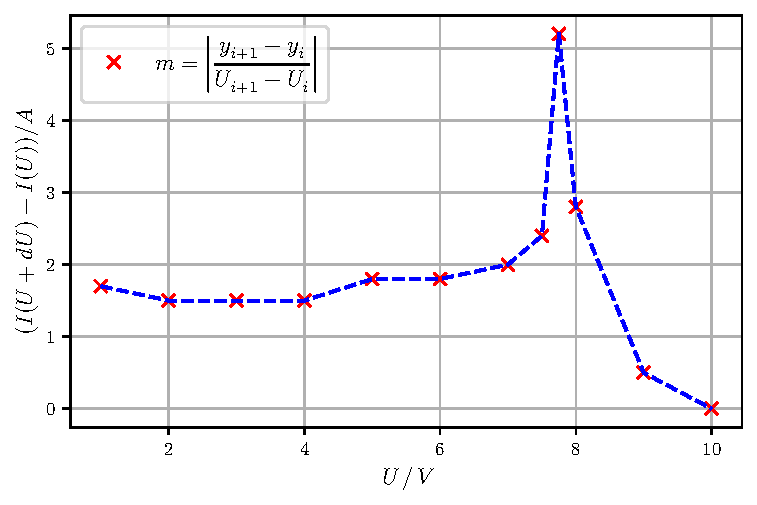
\includegraphics[width=\linewidth]{plot1.pdf}
  \caption{Die Messdaten sowie die Ausgleichsrechnung nach Gaußverteilung der Spannung in Abhängigkeit der Frequenz.}
  \label{fig:plot1}
\end{figure}
Aus \autoref{eq:gauss} ergeben sich die Parameter
\begin{align*}
  a &= \qty{1.98(15)}{\volt} \, ,\\
  b &= \num{6.1(1.2)} 
\end{align*}
und die zu bestimmenden Werte
\begin{align*}
  \nu_\text{0} = \qty{34.95}{kHz} \approx \qty{35}{kHz} &\quad \text{mit} \quad U_\text{A} = \qty{1.97}{\volt} \approx \qty{2}{\volt} \, .
\end{align*}


\subsection{Theoretische Bestimmung der Suszeptibilität}

